\subsection{Content Server} \label{section:counter-replace-server}
%START TEXT INPUT
This is my real text! Rest might be copied or not be checked!
%START TEXT INPUT

By introducing service managed account, the user has to login on a server in order for the application to work
an example is spotify, where the user logs in on a server and then can stream music
without account it is not possible to obtain the stream details and even though when the stream details are obtained they can be encrypted with a user specific key the attacker does not have
this way also an awesome algorithm can be moved onto the server that the application is only a thin client, this way reverse engineering or pirating does not offer any value to the attacker


\begin{figure}[h]
    \centering
    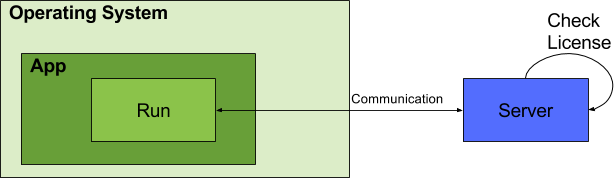
\includegraphics[width=0.8\textwidth]{data/contentServer.png}
    \caption{Abstraction of an application and a content server}
    \label{fig:contentServer}
\end{figure}


%eval
since the logic is on a server, luckyptahcer is not able to manipulate the logic, but it also has downsides
first of all the business model must be enabled to be put onto a server
in addition extra resources are needed, as knowledge and money to run a server, programm it and maintain two apps means twice the work
